\chapter{Pruebas del sistema}
En este cap�tulo se describen las principales pruebas realizadas con el robot de tal modo que sirva para validar el trabajo realizado y exponer a los resultados obtenidos.

\section{Simulaci�n con MobileSim}\label{MobileSim}
Una de las ventajas de utilizar el nodo rosaria para controlar el robot y obtener los datos de odometr�a es que las herramientas ofrecidas por el fabricante siguen pudiendo utilizarse. Este es el caso del simulador MobileSim.

MobileSim es un simulador rob�tico en dos dimensiones creado para los robots de Adpet Mobile Robots que puede utilizarse con robots controlados mediante la librer�a Aria.

Su funcionamiento es el siguiente: El simulador abre un puerto de comunicaci�n local en el ordenador y al ejecutar la conexi�n con el robot de Aria, si el robot no se encuentra se procede a conectarse a dicho puerto de comunicaci�n. Esto nos permite utilizar MobileSim con RosAria de la misma manera y sin cambiar nuestra configuraci�n.

\begin{figure}[htp]
\centering
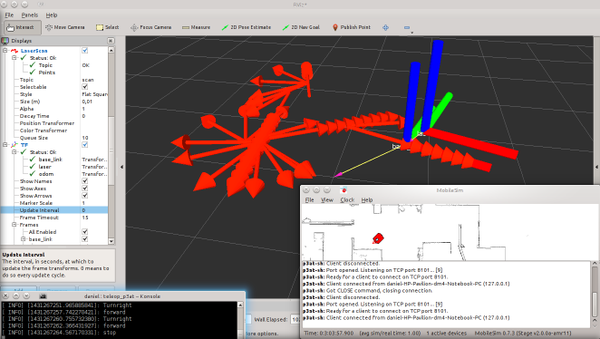
\includegraphics[width=0.5\textwidth]{figuras/mobilesim.png}
\caption{MobileSim junto con RViz funcionando con teleoperaci�n.}
\label{fig:mobilesim}
\end{figure}

Las pruebas con este simulador sirvieron para comprobar que el nodo rosaria dispon�a de la funcionalidad adecuada, as� como para realizar pruebas con el nodo de teleoperaci�n y dead\_reckoning.

Por otro lado, las limitaciones de este simulador son evidentes. No existe posibilidad de simular otros sensores incorporados al robot, la integraci�n de ROS se realiza con una librer�a intermedia y la m�s importante, no puede simularse un entorno en tres dimensiones.

\section{Simulaci�n con Gazebo}\label{Gazebo}
\subsection{SLAM}
\subsection{Datos de navegacion}

\section{Pruebas reales}
\subsection{SLAM}
\subsection{Datos de navegacion}
Test de resistencia
\subsection{Ascpectos de la navegaci�n}
